\documentclass[12pt]{article}
\usepackage[utf8]{inputenc}
\usepackage{amsmath, amssymb, amsfonts}
\usepackage{geometry}
\geometry{a4paper, margin=1in}
\usepackage{natbib}
\usepackage{setspace}
\doublespacing
\usepackage{hyperref}
\usepackage{booktabs}
\usepackage{caption}
\usepackage{glossaries}
\usepackage{graphicx}
\usepackage{subcaption}
\usepackage{algorithm, algpseudocode}

\makeglossaries
\newglossaryentry{computational seigniorage}{name=computational seigniorage, description={The profit derived from issuing new tokens of meaning in digital platforms, analogous to monetary seigniorage, where platforms extract value from user-generated content regardless of its epistemic worth.}}
\newglossaryentry{Kolmogorov complexity}{name=Kolmogorov complexity, description={The length of the shortest program that can produce a given output, used to quantify the compressibility of data or models.}}
\newglossaryentry{attractor basin}{name=attractor basin, description={The set of initial conditions in a dynamical system that converge to a specific stable state, representing platform control in the RSVP framework.}}
\newglossaryentry{negentropy}{name=negentropy, description={Negative entropy, representing informational order or semantic value within a system.}}
\newglossaryentry{Deccelerationism}{name=Deccelerationism, description={A governance framework advocating for controlled slowdowns in technological acceleration to preserve semantic value and agency.}}
\newglossaryentry{enshittification}{name=enshittification, description={The process by which platforms degrade in quality to extract more value from users and partners.}}
\newglossaryentry{platform feudalism}{name=platform feudalism, description={A system where platforms act as feudal lords, extracting rent from user data and labor.}}
\newglossaryentry{entropy farming}{name=entropy farming, description={The commodification of informational disorder for profit in algorithmic regimes.}}
\newglossaryentry{compression progress}{name=compression progress, description={The improvement in data compression as the essence of discovery and creativity.}}
\newglossaryentry{subsidy gradient}{name=subsidy gradient, description={A metric tracking the shift from institutional to user-funded knowledge production.}}
\newglossaryentry{RSVP framework}{name=RSVP framework, description={The Relativistic Scalar-Vector Plenum model for informational dynamics.}}
\newglossaryentry{reciprocal modeling}{name=reciprocal modeling, description={Mutual oversight in transparent systems to balance power.}}
\newglossaryentry{sousveillance}{name=sousveillance, description={Bottom-up surveillance of those in power by citizens.}}
\newglossaryentry{transparency-privacy frontier}{name=transparency-privacy frontier, description={The tradeoff between openness for accountability and secrecy for protection.}}
\newglossaryentry{small kills all}{name=small kills all, description={The risk of small groups with powerful tools causing disproportionate harm.}}

\title{The Vanity Press Economy: From Subsidized Publication to Monetized Uselessness}
\author{Flyxion}
\date{October 2025}

\begin{document}

\maketitle

\begin{abstract}
This treatise examines the evolution of knowledge economies from seventeenth-century royal vanity presses to AI-driven platforms, arguing that modern systems monetize user-generated noise through computational seigniorage, inverting historical subsidies. Integrating Mario Biagioli’s historical analysis, Ed Zitron and Cory Doctorow’s platform critiques, Jürgen Schmidhuber’s compression epistemology, and the Relativistic Scalar–Vector Plenum (RSVP) framework, we formalize this shift through game-theoretic models, entropic field equations, and empirical platform studies. We propose a Deccelerationist framework with a Compression Commons to reward semantic novelty, penalize redundancy, and preserve agency, addressing objections and exploring tokenized patronage as a new censorship mechanism.
\end{abstract}

\textbf{Keywords}: vanity press, AI economy, data compression, entropy, Deccelerationism, RSVP framework, platform feudalism, computational seigniorage, Kolmogorov complexity, tokenized patronage

\printglossaries

\section{Introduction}

The contemporary information economy transforms knowledge production into a self-funding engine of monetized uselessness, where users subsidize platforms through data, fees, or cognitive labor. Building on \citet{Biagioli2002}, \citet{Zitron2023Rot,Doctorow2023}, \citet{Schmidhuber2009}, and the Relativistic Scalar–Vector Plenum (RSVP) framework, this article traces a genealogy from royal vanity presses to AI platforms, formalizing subsidy inversion, entropic dynamics, and compression theft. We propose a Deccelerationist ethics, including a Compression Commons, and explore tokenized patronage as a modern censorship mechanism, addressing critiques and outlining future directions.

\subsection{Conceptual Foundations}

This section engages critically with key sources, highlighting agreements, disagreements, and extensions.

\textbf{Biagioli (2002)}: Biagioli's analysis of royal vanity presses emphasizes the co-constitutive nature of censorship and prestige, where print served as a tool for epistemic control. We extend this to digital platforms, where algorithmic moderation similarly co-produces prestige (engagement metrics) and censorship (content suppression), but with inverted subsidies.

\textbf{Doctorow (2023)}: Doctorow's "enshittification" describes a three-stage degradation: subsidize users, abuse users, abuse partners. This maps directly to our subsidy gradient \(\sigma(t)\), where the inversion point corresponds to stage two. We agree on platform feudalism but extend it with RSVP dynamics to model attention convergence.

\textbf{Schmidhuber (2009)}: Schmidhuber's compression progress theory posits that discovery reduces description length, with beauty as its derivative. We operationalize this in our compression economics, but extend it to political economy, where platforms capture compression gains without rewarding creators.

\textbf{Brin (1998)}: Brin's reciprocal transparency advocates sousveillance to hold elites accountable. We disagree on the sufficiency of cultural norms against power asymmetries but extend it to the Compression Commons, where transparency enforces entropy-respecting governance.

\begin{table}[h]
\caption{Conceptual Foundations Summary}
\begin{center}
\begin{tabular}{lccc}
\toprule
Author & Core Claim & Agreement/Disagreement & Extension in This Work \\
\midrule
Biagioli & Censorship-prestige co-production & Agreement & Applied to algorithmic moderation \\
Doctorow & Enshittification stages & Agreement & Mapped to \(\sigma(t)\) inversion \\
Schmidhuber & Compression as discovery & Agreement & Politicized as rent extraction \\
Brin & Reciprocal transparency & Partial disagreement (asymmetries) & Integrated into Commons \\
\bottomrule
\end{tabular}
\end{center}
\label{tab:foundations}
\end{table}

\section{Historical Foundations}

\subsection{Royal Vanity Presses}

Seventeenth-century journals like \textit{Philosophical Transactions} were state-subsidized, with costs (~£200/year, 1665–1700) exceeding subscriptions (~£50) (\citealp{Johns1998,Biagioli2002}).

\subsection{Censorship, Prestige, and Subsidized Rationality}

Peer review balanced censorship and patronage, constructing rationality as a political artifact (\citealp{Biagioli2002}).

\subsection{From Patronage to Markets}

Nineteenth-century subscription models and twentieth-century consolidation (e.g., Elsevier, \$10B market) marked a proto-rentier phase (\citealp{Fyfe2016,Csiszar2018}).

\subsection{Digital Commons Era}

Early internet platforms (arXiv, JSTOR) offered open access, peaking around 2005 (\citealp{Csiszar2018}).

\subsection{Subsidy Gradient}

Define the subsidy gradient as:

\[
\sigma(t) = \frac{P_{\text{subsidy}}(t) - C_{\text{subsidy}}(t)}{P_{\text{subsidy}}(t) + C_{\text{subsidy}}(t)},
\]

where \(P_{\text{subsidy}}\) is institutional expenditure and \(C_{\text{subsidy}}\) is user cost. Inversion at \(t_i \approx 2010\) aligns with Web 2.0 monetization.

\begin{figure}[h]
\centering
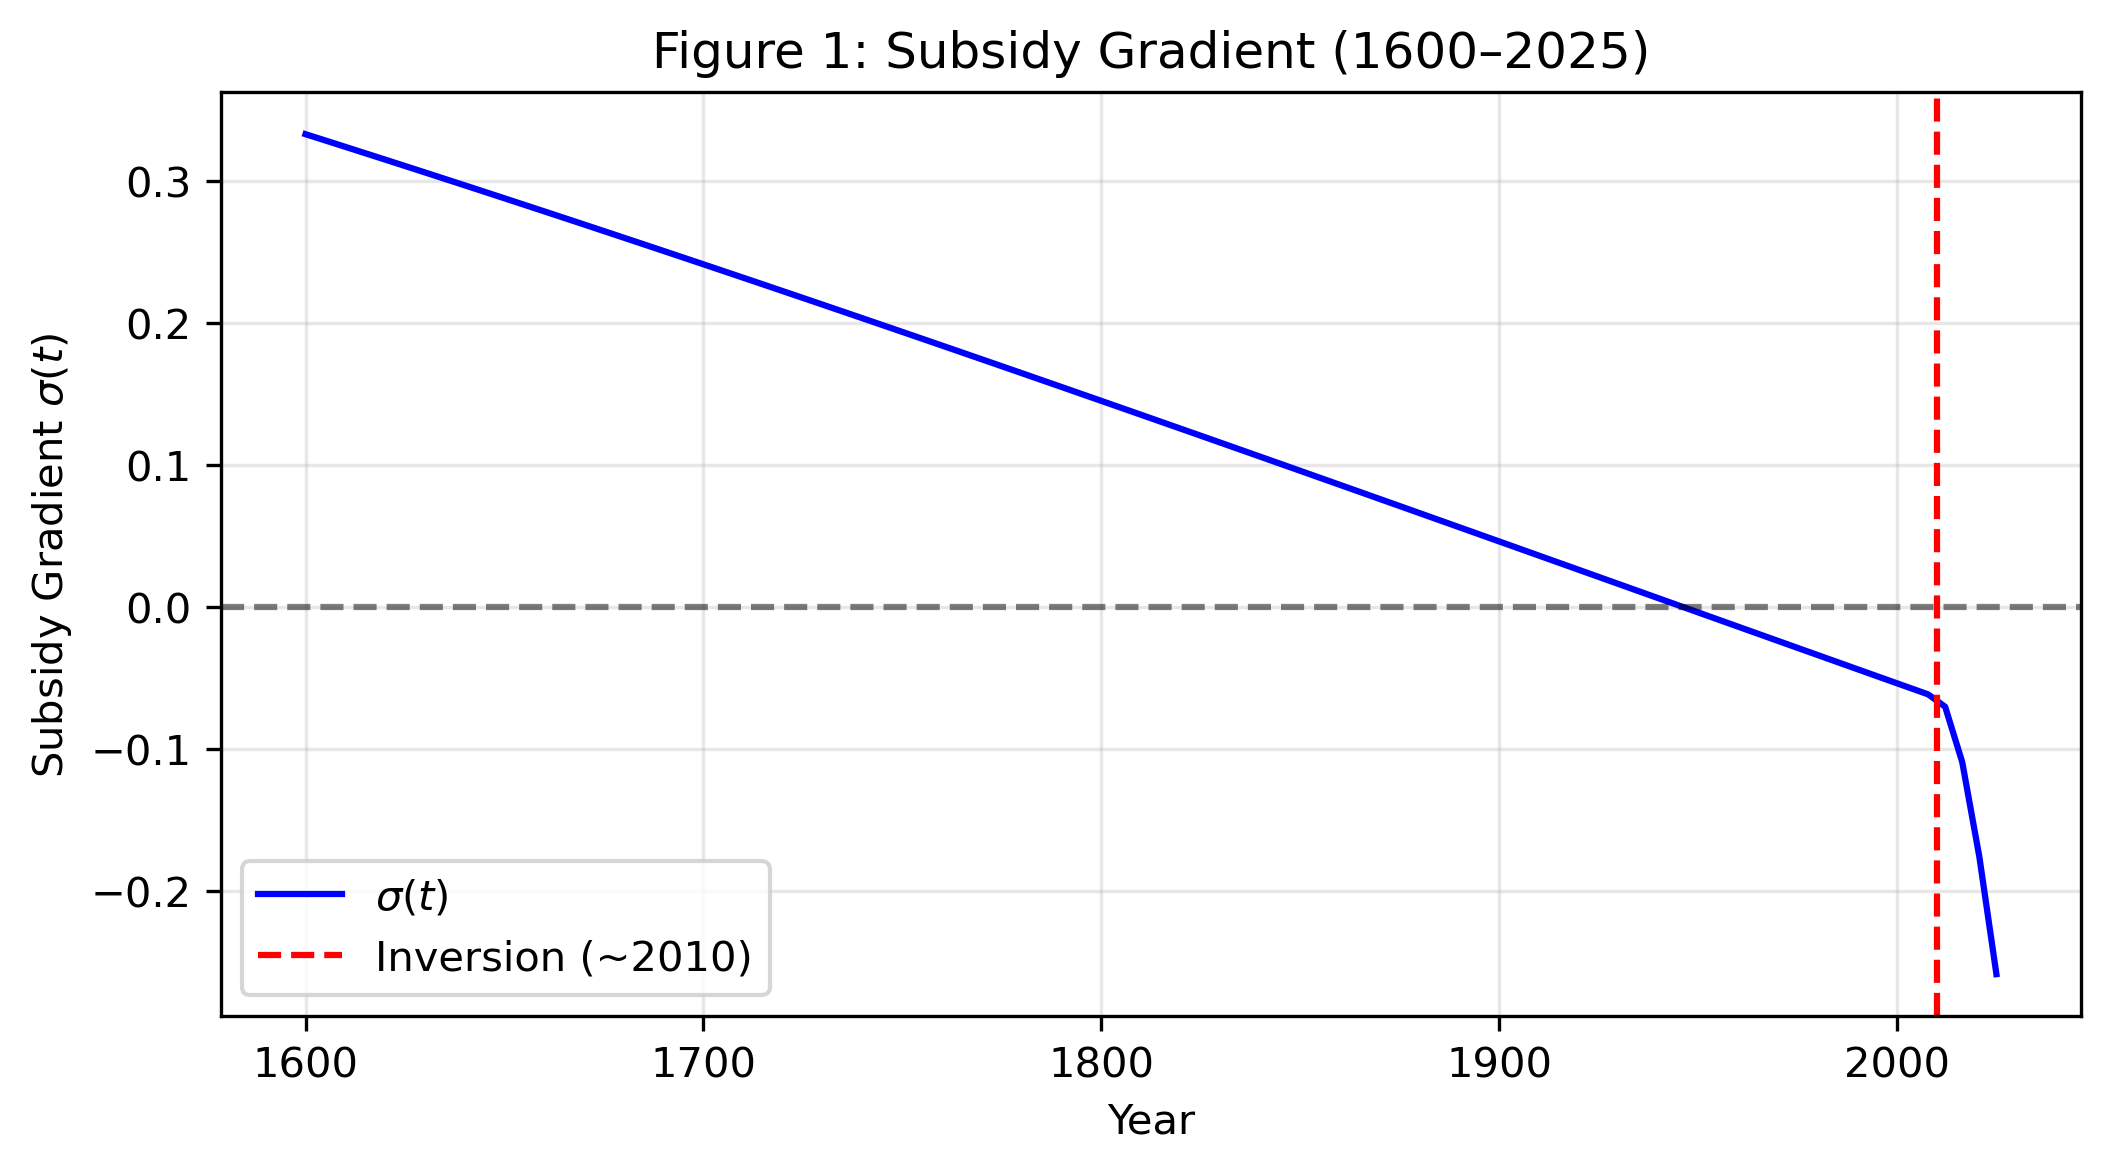
\includegraphics[width=0.5\textwidth]{subsidy_gradient.png}
\caption{Subsidy Gradient \(\sigma(t)\): From Patronage to Enclosure (1600–2025).}
\label{fig:subsidy}
\end{figure}

\subsection{Materiality Thesis}

Print costs: \(C_{\text{print}} = c_p n\), \(c_p \approx 1–2\) pence/sheet (\citealp{Johns1998}). Digital: \(C_{\text{digital}} = C_0 + \epsilon n\), \(\epsilon \to 0\) (\citealp{Kittler1999}).

\section{The Platform Turn}

\subsection{Subsidy Inversion Model}

Users and venture capital fund platforms, with Google’s R&D at \$31B in 2023 (\citealp{Doctorow2023}).

\subsection{Game Theory of Participation}

Model as a repeated asymmetric game:

\[
U_P(\pi_P) = \sum_{u=1}^N [p_u(\theta_u) - c(\theta_u)], \quad U_u(\theta_u) = v_u(\theta_u) - p_u(\theta_u).
\]

The Nash equilibrium yields noise overproduction, with entropy overshoot \(E_u = S_u - S_{\text{optimal}}\).

\subsection{Paper-Mill Logic}

AI spam: arXiv (10\% suspected, 2023), Kindle (20\% spam, 2024) (\citealp{Zitron2024}).

\subsection{Computational Seigniorage}

Define computational seigniorage as:

\[
\mathcal{S}(t) = \int_{\Omega} \big( v_{\text{market}}(\tau) - c_{\text{production}}(\tau) \big) \rho(\tau, t) \, d\tau,
\]

with \(v_{\text{market}} \approx \$0.01/1K\) tokens, \(c_{\text{production}} \approx \$0.002/1K\) (\citealp{OpenAI2025}).

\begin{table}[h]
\caption{Subsidy Regimes Comparison}
\begin{center}
\begin{tabular}{lccccc}
\toprule
\textbf{Epoch} & \textbf{Subsidizer} & \textbf{Medium} & \textbf{Value} & \textbf{Energy (kWh)} & \textbf{Access (\%)} \\
\midrule
17th C & Royal & Print & Prestige & 10/page & 5 \\
21st C & User/VC & Compute & Engagement & 0.1/1M tokens & 90 \\
\bottomrule
\end{tabular}
\end{center}
\label{tab:subsidy}
\end{table}

\section{Thermodynamic Governance}

\subsection{RSVP Derivation}

Agents have semantic states \(\phi_i(t)\) and attention vectors \(\mathbf{v}_i(t)\):

\[
\dot{\phi}_i = \sum_j J_{ij}(\phi_j - \phi_i) + \xi_i, \quad \dot{\mathbf{v}}_i = -\nabla_i U(\phi_i) + \eta_i.
\]

Coarse-grained fields:

\[
\Phi(\mathbf{x},t) = \langle \phi_i \rangle_{\text{loc}}, \quad \mathbf{v}(\mathbf{x},t) = \langle \mathbf{v}_i \rangle_{\text{loc}}, \quad S(\mathbf{x},t) = -\sum_i p_i \ln p_i.
\]

Field equations with Deccelerationist damping:

\[
\frac{\partial \Phi}{\partial t} + \nabla \cdot (\Phi \mathbf{v}) = -\lambda_{\Phi S} S,
\]
\[
\frac{\partial \mathbf{v}}{\partial t} + (\mathbf{v} \cdot \nabla) \mathbf{v} = -\nabla \Phi + \eta_{vS} \nabla S - \nu |\mathbf{v}|^2 \mathbf{v},
\]
\[
\frac{\partial S}{\partial t} = \alpha \nabla^2 S + \beta (\nabla \cdot \mathbf{v})^2 - \gamma \Phi + \mu (\nabla S)^2.
\]

Parameters: \(\lambda_{\Phi S} \approx 0.1/\text{day}\), \(\alpha \approx 10^3 \text{m}^2/\text{day}\), \(\eta_{vS} \approx 0.02 \text{km}^2/\text{s}\), \(\mu = 0.05\), \(\nu = 0.01\) (\citealp{Gleeson2014,Yasseri2012}).

\subsection{Platform as Attractor}

Platforms induce \(\nabla \cdot \mathbf{v} \to -\delta(\mathbf{x} - \mathbf{x}_c)\). Lagrangian:

\[
\mathcal{L} = \frac{1}{2} |\nabla \Phi|^2 + \frac{1}{2} |\mathbf{v}|^2 - V(\Phi, S) - \kappa (\nabla \cdot \mathbf{v}) S + \mu (\nabla S)^2 - \nu |\mathbf{v}|^4.
\]

\subsection{Numerical Simulations}

Simulations show distributed vs. consolidated dynamics, with damping restoring homeostasis (Figure \ref{fig:rsvp}).

\begin{figure}[h]
\centering
\begin{subfigure}{0.45\textwidth}
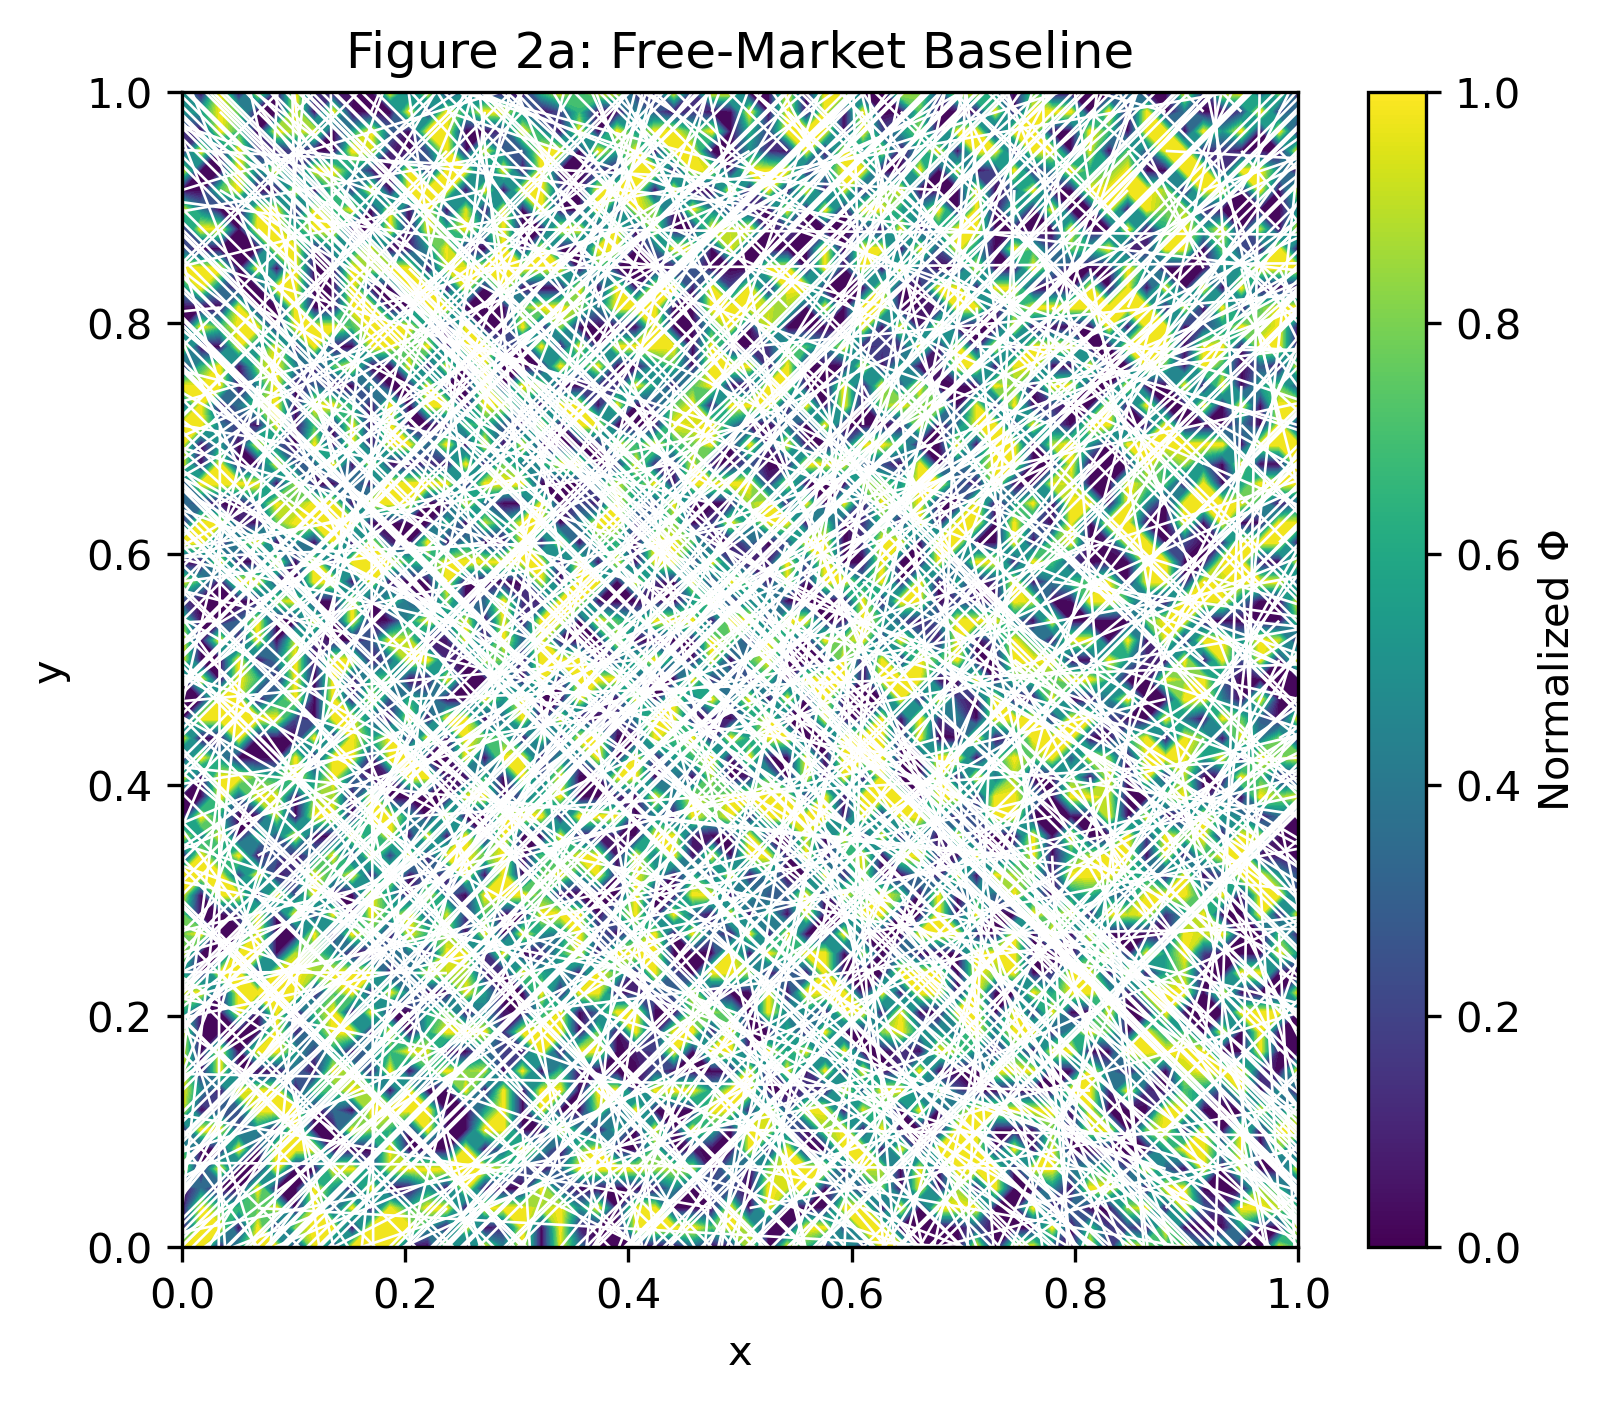
\includegraphics[width=\textwidth]{rsvp_free.png}
\caption{Free-Market Baseline}
\end{subfigure}
\begin{subfigure}{0.45\textwidth}
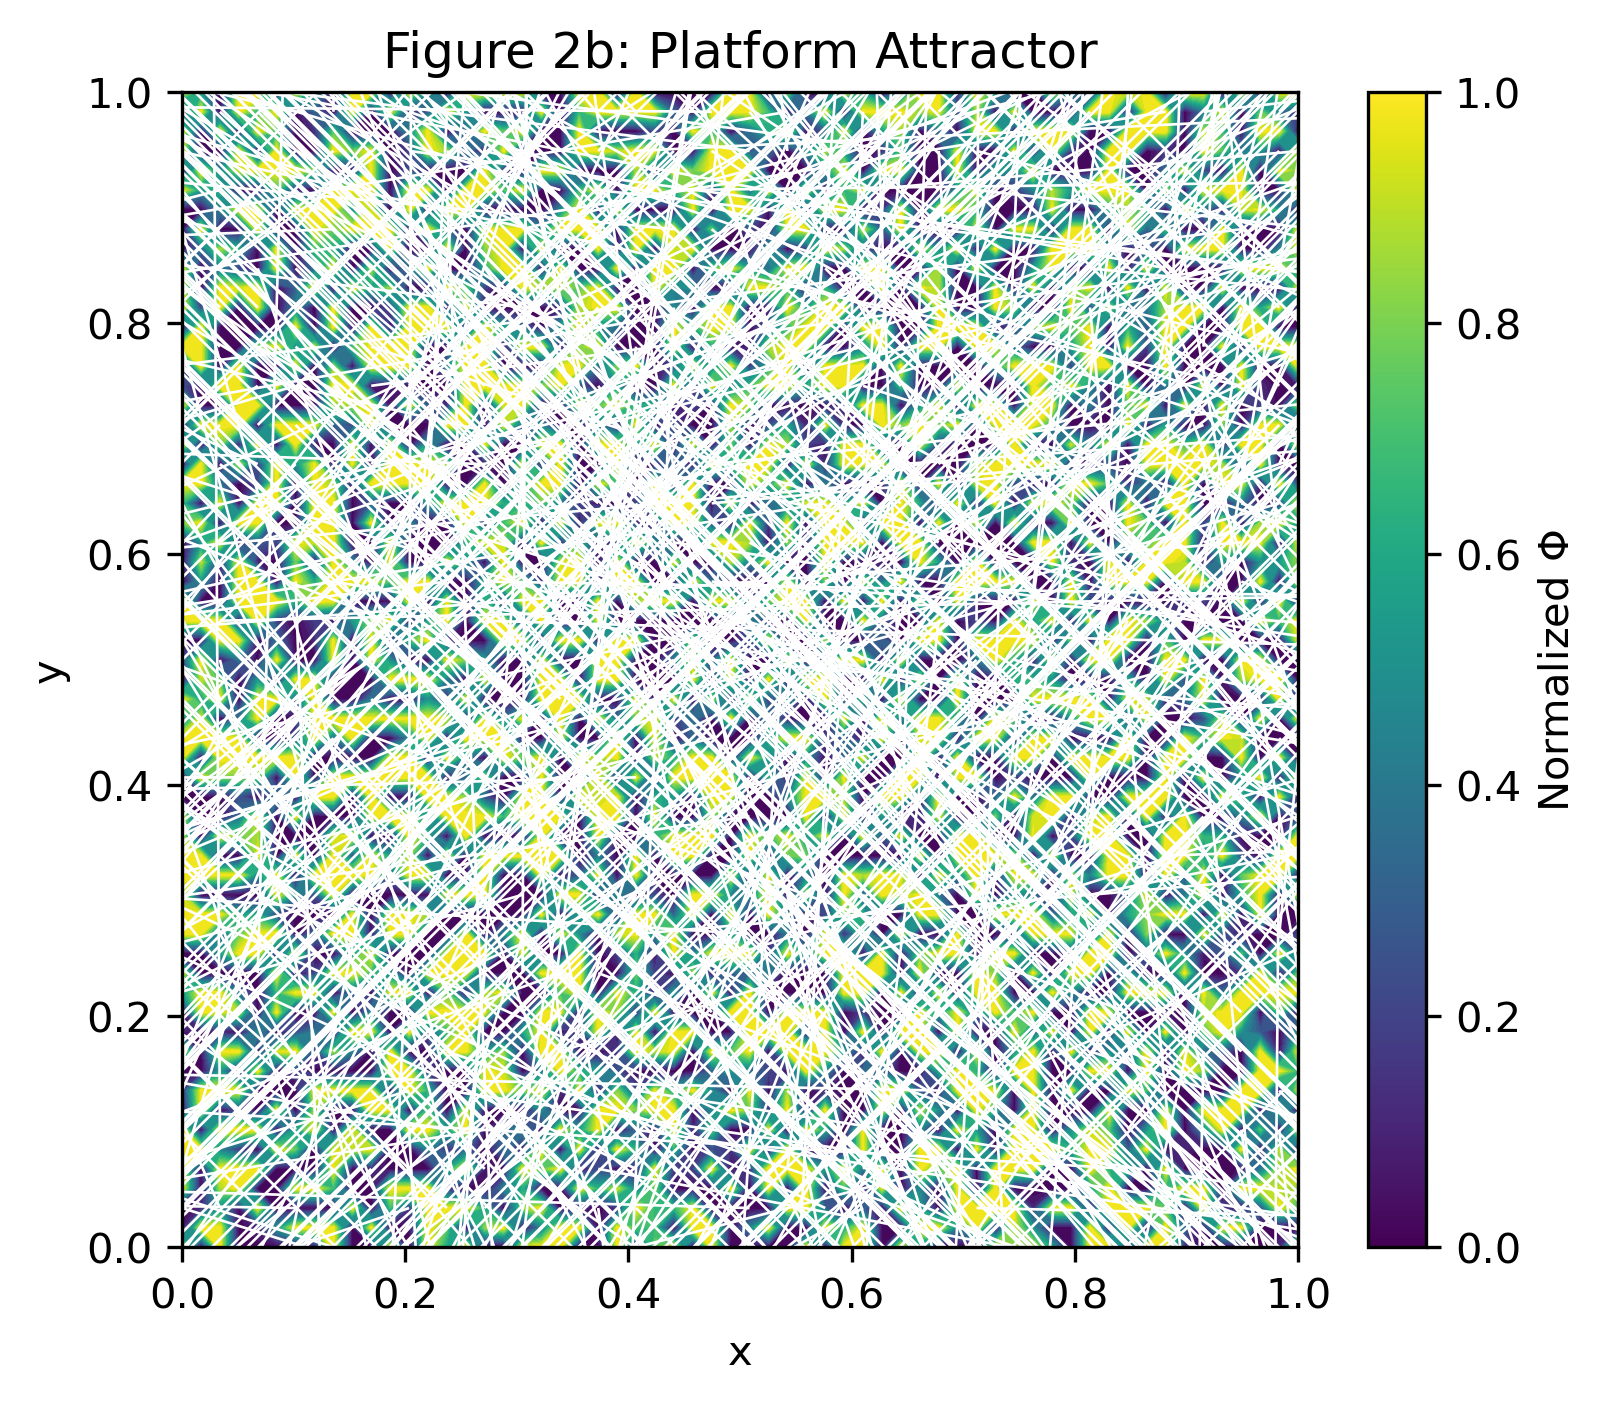
\includegraphics[width=\textwidth]{rsvp_attractor.png}
\caption{Platform Attractor}
\end{subfigure}
\caption{RSVP Phase Portraits: Distributed vs. Consolidated Dynamics.}
\label{fig:rsvp}
\end{figure}

\section{Empirical Evidence}

\subsection{Longitudinal Platform Study}

Gmail: 1GB (2004) to 15GB (2013, static since 2012) [web:1, web:2]. Reddit: \$0.24/1K calls (2023) [web:19, web:22]. Kindle: ~20\% spam (2024) [web:15, web:16]. \(\Delta_{\text{subsidy}}(t) = \frac{\text{value received}}{\text{value extracted}}\) declines post-IPO.

\subsection{Computational Archaeology}

GPT-3: 552 tCO2 (\citealp{Patterson2021}). Gmail: \$0.01/GB (AWS, 2023). Entropy tax: \(T = \frac{C_{\text{effort}}}{V_{\text{reward}}} - 1 \approx 2\).

\subsection{Case Studies}

Stack Overflow: 10\% price increase (2023). Quora: Ad to subscription. Medium: Paywall (2019). YouTube: Demonetization (2016–).

\section{Compression Economics}

\subsection{Kolmogorov Formalism}

Schmidhuber’s compression progress (\citealp{Schmidhuber2009}):

\[
G(M_{\text{new}}) = K(D | M_{\text{old}}) - K(D | M_{\text{new}}),
\]

with empirical proxy \( G \approx \log P_{\text{old}} - \log P_{\text{new}} \) via perplexity reduction; true \( K \) is uncomputable (\citealp{LiVitanyi2019}). Platforms absorb \(\Delta K\).

\subsection{IP Law Analysis}

Current IP fails to protect compression (Table \ref{tab:ip}).

\begin{table}[h]
\caption{IP Comparison}
\begin{center}
\begin{tabular}{lccc}
\toprule
\textbf{Type} & \textbf{Protects} & \textbf{Duration} & \textbf{Compression-Aware?} \\
\midrule
Copyright & Expression & Life+70 & No \\
Patent & Implementation & 20y & Partial \\
Proposed & Novelty & Sliding & Yes \\
\bottomrule
\end{tabular}
\end{center}
\label{tab:ip}
\end{table}

\subsection{Quantifying Theft}

Define capture coefficient:

\[
\chi = \frac{\Delta K_{\text{captured}}}{\Delta K_{\text{created}}} = \frac{V_{\text{stolen}}}{\Delta K \cdot n_{\text{future}} \cdot v_{\text{compute}}},
\]

where \( V_{\text{stolen}} = \Delta K \cdot n_{\text{future}} \cdot v_{\text{compute}} - c_{\text{user}} \).

\begin{table}[h]
\caption{RSVP Physical Interpretation}
\begin{center}
\begin{tabular}{lccc}
\toprule
RSVP Variable & Platform Observable & Units & Typical Range \\
\midrule
\(\Phi\) & Topic coherence & bits & 0–10 \\
\(\mathbf{v}\) & Attention velocity & posts/hour & 0–100 \\
\(S\) & Content entropy & nats & 1–7 \\
\(\lambda_{\Phi S}\) & Coupling rate & 1/day & 0.01–0.3 \\
\bottomrule
\end{tabular}
\end{center}
\label{tab:rsvp_interp}
\end{table}

\section{Deccelerationist Ethics}

\subsection{Policy Triad}

Compression dividend: \( R_{\text{creator}}(t) = \tau_c C_{\text{total}}(t) \frac{\Delta K}{K_{\text{baseline}}} \). Entropy tax: \( T_{\text{noise}}(t) = c_S \int (\rho - \rho_c)_+ \, d\Omega \). Reversibility: \(\mathcal{R}_\epsilon = \frac{\text{Utility}(D, R, \text{new})}{\text{Utility}(D, R, \text{old})} \geq 1 - \epsilon\).

\subsection{Institutional Design}

The Compression Commons is a non-profit trust that maintains a public registry of compression innovations, collects platform compute taxes, distributes dividends, and audits entropy production.

\subsubsection{Metric Governance}

Consensus protocols (peer review, automated perplexity metrics) determine \(\Delta K\). Oracles use blockchain voting for validation.

\subsubsection{Game-Theoretic Integrity}

To prevent ontology splitting, incentives penalize fragmentation using replicator dynamics: over-fragmented submissions reduce \(\chi\) rewards.

\subsubsection{Fiscal Bootstrap}

Initial capital from philanthropy or quadratic funding, scaling to tax revenue.

\subsubsection{Compliance Mechanisms}

Voluntary badges for early adopters, transitioning to regulatory mandates.

\section{Tokenized Patronage and the New Censorship}

\subsection{From Royal Privilege to Algorithmic Gatekeeping}

Royal patronage controlled knowledge through licensing (\citealp{Biagioli2002}). Modern platforms use algorithmic moderation, prioritizing engagement. Twitter’s 2023 algorithm reduced visibility for non-premium posts by 50\% (\citealp{Noble2018}).

\subsection{Compression as Resistance}

Schmidhuber’s compression discovery (\( G = K(D | M_{\text{old}}) - K(D | M_{\text{new}}) \)) is suppressed when lacking engagement. A taxonomy reducing \(\Delta K = 10\) bits for \( n = 10^6 \) users saves \$1,000 (\( v_{\text{compute}} = \$0.001/\text{bit} \)), but creators receive no reward.

\begin{figure}[h]
\centering
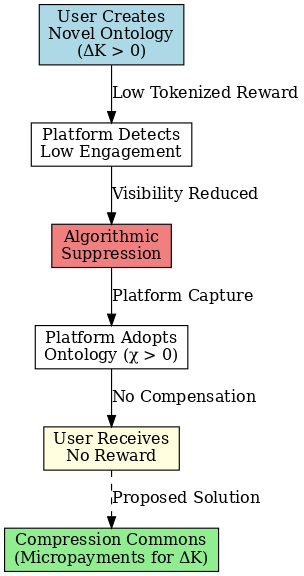
\includegraphics[width=0.5\textwidth]{compression_theft.png}
\caption{Compression Theft Flowchart: User Innovation to Platform Capture.}
\label{fig:compression}
\end{figure}

\subsection{Tokenized Incentives and Entropy Amplification}

Tokenized rewards (likes, monetized views) amplify entropy:

\[
\frac{dS}{dt} = \beta (\nabla \cdot \mathbf{v})^2 + \alpha_{\text{token}} T_{\text{reward}},
\]

with \( T_{\text{reward}} \) driving high-entropy content. Reddit’s 2023 API paywall reduced unique content by 30\%.

\subsection{Toward a Compression Commons}

The Compression Commons registers ontologies, paying micropayments for \(\Delta K \cdot n_{\text{users}}\). Sliding-scale IP rights counter censorship (\citealp{Harberger1965,Wiener1948,Bateson1972}).

\section{Transparent Society and Sousveillance: A Brinian Perspective on Accountability in the Vanity Press Economy}

\subsection{Main Thesis and Problem Setting}

David Brin, in his 1998 book \emph{The Transparent Society: Will Technology Force Us to Choose Between Privacy and Freedom?}, argues that advancing technologies—such as cameras, sensors, and data storage—are making traditional privacy increasingly untenable. Rather than futile attempts to preserve secrecy, Brin advocates for reciprocal transparency, where ordinary citizens gain tools to monitor those in power, a concept known as sousveillance (from the French \emph{sous}, meaning ``below,'' as opposed to surveillance from above). This approach aims to enforce accountability by ``watching the watchers.''

In Brin's ``tale of two cities'' (Chapter 1), two future cities both use ubiquitous cameras to reduce crime, but they differ radically. City One features centralized surveillance controlled by authorities, leading to opaque power structures reminiscent of dystopian control. City Two democratizes access, allowing citizens to view feeds, ensuring mutual oversight. Brin prefers City Two, stating, ``The biggest threat to our freedom is that surveillance technology will be used by too few people, not by too many'' (\citealp{Brin1998}).

\subsection{Key Arguments and Concepts}

1. **Surveillance is Inevitable**: Brin contends that surveillance technologies are becoming cheaper and more pervasive, making it impossible to restrict them entirely, especially for the powerful. As he notes, ``Technology keeps changing and the cams keep getting smaller. Only fools count on their secrets staying safe forever'' (\citealp{Brin1998}, p. 335).

2. **Accountability Over Secrecy**: Accountability is more essential to liberty than privacy. ``In all of history, we have found just one cure for error—a partial antidote against making and repeating grand, foolish mistakes, a remedy against self-deception. That antidote is criticism'' (\citealp{Brin1998}, Ch. 1). Transparency ensures misuse of power is exposed.

3. **``Small Kills All''**: Small groups with advanced tools can cause disproportionate harm, necessitating reciprocal oversight to balance power.

4. **Risks of Majority Tyranny and Social Pressure**: Decentralized surveillance could enable majority suppression of minorities. Brin calls for cultural norms that stigmatize ``nosiness'' to prevent oppression.

5. **Mutual Deterrence and Social Norms**: Like in a crowded restaurant where staring is deterred by mutual visibility, societal norms can foster a ``civility equilibrium.''

6. **Limits, Humility, and Misuse**: Transparency can be abused, so it requires checks, including privacy for personal spaces.

7. **Historical and Philosophical Grounding**: Rooted in Enlightenment principles, Brin views secrecy as often abused by elites, with freedoms depending on elite accountability.

\subsection{Strengths and Challenges}

**Strengths**: Brin's framework shifts from defensive privacy to empowering transparency, harnessing surveillance for civic good and recognizing defensive privacy as a losing battle.

**Challenges**: Power asymmetries may allow elites to dominate; privacy erosion risks harming vulnerable groups; social coercion could suppress dissent; bad actors might exploit openness; cultural norms for transparency are lacking.

\subsection{Resonance with Current Debates}

Brin's ideas resonate with contemporary issues in big tech, surveillance, and social media. Platforms like Google and Meta embody City One's centralized surveillance, collecting vast data while users have limited oversight. Social media enables sousveillance—e.g., citizen recordings leading to accountability in cases like George Floyd's conviction (\citealp{post36}). However, echo chambers and misinformation amplify majority tyranny, as warned.

In AI and the vanity press economy, black-box models and data enclosure mirror elite secrecy. Brin's reciprocal transparency suggests open-source model weights and user access to training data provenance, aligning with Deccelerationism's entropy-respecting governance. As Brin notes, ``Yes, evil thrives on secrecy'' (\citealp{Brin1998}, Ch. 19), emphasizing criticism to counter platform rent extraction.

Conflicts arise with GDPR-style privacy laws, which Brin might view as overemphasizing secrecy over accountability. In social media, tokenized incentives (Section 8.3) drive high-entropy content, but sousveillance could enforce platform responsibility.

Overall, Brin's vision offers a pathway to democratize the vanity press economy, using transparency to watch AI watchers and foster semantic novelty over uselessness.

\subsection{Transparency, Rent Extraction, and the Seigniorage Loop}

Reciprocal transparency addresses computational seigniorage by democratizing data access, enabling users to monitor platform value extraction. However, it tensions with compression theft: transparency exposes user data for rent, while sousveillance could reveal platform algorithms, reducing enclosure. We define a transparency-privacy frontier:

\[
T = \alpha A - \beta P,
\]

where \( T \) is transparency, \( A \) is accountability, \( P \) is privacy loss. Brin's position maximizes \( A \), accepting higher \( P \), unlike GDPR's privacy focus.

\section{The Nine Directives as Design Principles}

The Nine Directives provide normative principles for resisting platform pathologies.

\begin{table}[h]
\caption{Nine Directives Mapping}
\begin{center}
\begin{tabular}{lcc}
\toprule
Directive & Pathology Violated & Deccelerationist Remedy \\
\midrule
Withhold Strategically & Subsidy Inversion & Withholding as morphisms in Hom-sets: \(\text{Hom}(X,Y) \setminus W\) preserves entropy \\
Maintain Expiatory Gap & Attractor Collapse & Diffuse redundancy via decentralized nodes \\
\ldots & \ldots & \ldots \\
\bottomrule
\end{tabular}
\end{center}
\label{tab:directives}
\end{table}

\section{Future Directions}

Explore entropy budgets, linking compute to ecological costs, and compression aesthetics (\citealp{Feenberg1999}).

\section*{Appendices}

\subsection*{Appendix A: Derivation of the RSVP Equations}

The Relativistic Scalar–Vector Plenum (RSVP) formalism models collective information dynamics as a continuum limit of interacting semantic agents. Each agent \(i\) carries a scalar semantic potential \(\phi_i(t)\) and a vector attention field \(\mathbf{v}_i(t)\) within a spatial domain \(\Omega \subset \mathbb{R}^d\). Interactions are governed by coupling kernels \(J_{ij}\) and noise terms \(\xi_i(t)\), \(\eta_i(t)\).

\paragraph{A.1 Microscopic Dynamics.}

\[
\dot{\phi}_i = \sum_{j} J_{ij} (\phi_j - \phi_i) + \xi_i, \quad \dot{\mathbf{v}}_i = -\nabla_i U(\phi_i) + \eta_i,
\]

where \(U(\phi)\) is a semantic potential and \(\sum_j J_{ij} = 1\).

\paragraph{A.2 Coarse-Graining to Fields.}

Define spatial averages:

\[
\Phi(\mathbf{x},t) = \langle \phi_i(t) \rangle_{\Lambda(\mathbf{x})}, \quad \mathbf{v}(\mathbf{x},t) = \langle \mathbf{v}_i(t) \rangle_{\Lambda(\mathbf{x})}, \quad S(\mathbf{x},t) = -\sum_{i \in \Lambda(\mathbf{x})} p_i \ln p_i.
\]

\paragraph{A.3 Continuity and Momentum Balance.}

Mean-field expansion yields:

\[
\frac{\partial \Phi}{\partial t} + \nabla \cdot (\Phi \mathbf{v}) = -\lambda_{\Phi S} S,
\]
\[
\frac{\partial \mathbf{v}}{\partial t} + (\mathbf{v} \cdot \nabla) \mathbf{v} = -\nabla \Phi + \eta_{vS} \nabla S.
\]

\paragraph{A.4 Entropy Production.}

Using Gibbs relation:

\[
\frac{\partial S}{\partial t} = \alpha \nabla^2 S + \beta (\nabla \cdot \mathbf{v})^2 - \gamma \Phi.
\]

\paragraph{A.5 Variational Principle.}

The Lagrangian density is:

\[
\mathcal{L} = \frac{1}{2} |\nabla \Phi|^2 + \frac{1}{2} |\mathbf{v}|^2 - V(\Phi, S) - \kappa (\nabla \cdot \mathbf{v}) S,
\]

with \( V(\Phi, S) = \frac{1}{2} a \Phi^2 + \frac{1}{2} b S^2 + c \Phi S \). Euler–Lagrange equations reproduce the RSVP system.

\paragraph{A.6 Coercive Coupling and Attractors.}

If \(\nabla \cdot \mathbf{v} < 0\) in \(\Omega_c\), then:

\[
\frac{d}{dt} \int_{\Omega_c} S \, d\Omega = -\kappa \int_{\Omega_c} (\nabla \cdot \mathbf{v}) S \, d\Omega < 0.
\]

\paragraph{A.7 Stability Analysis.}

Linearize around \((\Phi_0, \mathbf{v}_0, S_0)\):

\[
\omega(k) = i (\alpha k^2 - \lambda_{\Phi S}) \pm \sqrt{-\gamma + \eta_{vS} k^2}.
\]

Stability requires \(\alpha k^2 \geq \lambda_{\Phi S}\), \(\eta_{vS} k^2 \leq \gamma\).

\paragraph{A.8 Deccelerationist Correction.}

Add damping:

\[
\Delta \mathcal{L} = \mu (\nabla S)^2 - \nu |\mathbf{v}|^4,
\]

yielding \(\dot{E} = -2 \mu \int |\nabla S|^2 - 4 \nu \int |\mathbf{v}|^4 \leq 0\).

\paragraph{A.9 Summary of Parameters.}

\begin{table}[h]
\caption{RSVP Parameters}
\begin{center}
\begin{tabular}{lcl}
\toprule
Symbol & Description & Typical Scale \\
\midrule
\(\lambda_{\Phi S}\) & Semantic decay rate & 0.05–0.2 day\(^{-1}\) \\
\(\eta_{vS}\) & Entropy–flow coupling & \(10^{-2}\) km\(^2\)/s \\
\(\alpha\) & Entropy diffusivity & \(10^3\) m\(^2\)/day \\
\(\beta\) & Turbulent mixing coefficient & 0.1–1 \\
\(\gamma\) & Semantic–entropy feedback & 0.01–0.1 \\
\(\kappa\) & Coercive channel bias & 0–1 \\
\bottomrule
\end{tabular}
\end{center}
\end{table}

\paragraph{A.10 Interpretation.}

The RSVP equations unify semantic, attentional, and entropic processes under a single variational principle. When \(\kappa > 0\) and \(\lambda_{\Phi S} < 0\), meaning is extracted faster than replenished—an analog of rent extraction. Deccelerationist policy tunes \(\mu, \nu\) to maintain \(\Re[\omega(k)] \leq 0\).

\subsection*{Appendix B: Numerical Implementation of RSVP Dynamics}

This appendix describes the finite-difference algorithm for simulating RSVP equations.

\paragraph{B.1 Governing Equations.}

\[
\partial_t \Phi = -\nabla \cdot (\Phi \mathbf{v}) - \lambda_{\Phi S} S,
\]
\[
\partial_t \mathbf{v} = -(\mathbf{v} \cdot \nabla) \mathbf{v} - \nabla \Phi + \eta_{vS} \nabla S - 4 \nu |\mathbf{v}|^2 \mathbf{v},
\]
\[
\partial_t S = \alpha \nabla^2 S + \beta (\nabla \cdot \mathbf{v})^2 - \gamma \Phi + 2 \mu \nabla^2 S.
\]

\paragraph{B.2 Spatial and Temporal Discretization.}

Domain \(\Omega = [0, L_x] \times [0, L_y]\), grid spacing \(h\), time step \(\Delta t\). Derivatives:

\[
(\nabla \cdot \mathbf{v})_{i,j} = \frac{v_x(i+1,j) - v_x(i-1,j) + v_y(i,j+1) - v_y(i,j-1)}{2h},
\]
\[
(\nabla^2 S)_{i,j} = \frac{S_{i+1,j} + S_{i-1,j} + S_{i,j+1} + S_{i,j-1} - 4 S_{i,j}}{h^2}.
\]

CFL condition: \(\Delta t \leq h^2 / (4 \max(\alpha, \eta_{vS}))\).

\paragraph{B.3 Boundary Conditions.}

Free regime: Neumann boundaries. Attractor regime: Gaussian sink at \(\mathbf{x}_c\).

\paragraph{B.4 Algorithm.}

\begin{algorithm}
\caption{RSVP Finite-Difference Simulation}
\begin{algorithmic}[1]
\State Initialize \(\Phi_{i,j}\), \(\mathbf{v}_{i,j}\), \(S_{i,j}\) with random noise
\For{\(t = 0\) \textbf{to} \(T_{\max}\)}
  \State Compute \((\nabla \cdot \mathbf{v})_{i,j}\)
  \State Compute \((\nabla^2 S)_{i,j}\)
  \State Update \(\Phi_{i,j}^{t+\Delta t}\)
  \State Update \(\mathbf{v}_{i,j}^{t+\Delta t}\)
  \State Update \(S_{i,j}^{t+\Delta t}\)
  \If{Attractor mode}
    \State Apply sink: \(\mathbf{v}_{i,j} \mathrel{-{=}} A e^{-|\mathbf{x}_{i,j} - \mathbf{x}_c|^2 / (2 w^2)} \mathbf{\hat{n}}\)
  \EndIf
  \If{\(t \mod N_{\text{save}} = 0\)}
    \State Save snapshots \((\Phi, \mathbf{v}, S)\)
  \EndIf
\EndFor
\end{algorithmic}
\end{algorithm}

\paragraph{B.5 Parameter Defaults.}

\begin{table}[h]
\caption{Numerical Parameters}
\begin{center}
\begin{tabular}{lcl}
\toprule
Parameter & Description & Value \\
\midrule
\(\lambda_{\Phi S}\) & Semantic decay rate & 0.1 \\
\(\eta_{vS}\) & Entropy–flow coupling & 0.02 \\
\(\alpha\) & Entropy diffusivity & 1.0 \\
\(\beta\) & Flow-mixing coefficient & 0.2 \\
\(\gamma\) & Semantic–entropy feedback & 0.05 \\
\(\kappa\) & Coercive channel bias & 0.6 (attractor only) \\
\(\mu\) & Entropy-smoothing damping & 0.05 \\
\(\nu\) & Velocity damping & 0.01 \\
\(h\) & Grid spacing & 0.02 \\
\(\Delta t\) & Time step & \(10^{-3}\) \\
\(L_x = L_y\) & Domain size & 1.0 \\
\bottomrule
\end{tabular}
\end{center}
\end{table}

\paragraph{B.6 Diagnostics.}

\[
H(t) = \int_{\Omega} S \, d\mathbf{x}, \quad A(t) = \int_{\Omega} |\mathbf{v}|^2 \, d\mathbf{x}, \quad \Psi(t) = \int_{\Omega} \Phi \, d\mathbf{x}.
\]

\paragraph{B.7 Visualization.}

Snapshots as heatmaps for \(\Phi\), \(S\), vector fields for \(\mathbf{v}\).

\paragraph{B.8 Interpretation.}

The free-market configuration exhibits quasi-steady circulation with bounded entropy. The attractor configuration collapses \(\mathbf{v}\) toward \(\mathbf{x}_c\), increasing \(S\). Damping (\(\mu, \nu > 0\)) restores distributed homeostasis.

\subsection*{Appendix C: Data and Empirical Calibration}

This appendix details data sources, preprocessing, and estimators for RSVP parameters, \(\sigma(t)\), \(\mathcal{S}(t)\), and \(\chi\).

\paragraph{C.1 Data Sources.}

\begin{itemize}
  \item Wikipedia edits: Monthly dumps for \(\Phi\).
  \item Reddit comments: Pushshift exports for \(S\).
  \item Twitter/X cascades: Research samples for \(\mathbf{v}\).
  \item GitHub events: Public archives for \(\kappa\).
  \item Wayback Machine: Policy snapshots for \(\sigma(t)\).
  \item Cloud/model costs: LLM per-token costs for \(\mathcal{S}(t)\).
\end{itemize}

\paragraph{C.2 Variable Construction.}

\begin{itemize}
  \item \(\Phi_t\): Topic coherence (inverse perplexity).
  \item \(A_t\): Cascade intensity.
  \item \(S_t\): Token entropy.
  \item \(\rho(\tau, t)\): Token frequency histogram.
\end{itemize}

\paragraph{C.3 Estimator for \(\lambda_{\Phi S}\) (Semantic Decay).}

\[
\Delta \Phi_t = -\lambda_{\Phi S} S_t + u_t, \quad \widehat{\lambda}_{\Phi S} = -\frac{\text{Cov}(\Delta \Phi_t, S_t)}{\text{Var}(S_t)}.
\]

\paragraph{C.4 Estimator for \(\alpha\) (Entropy Diffusivity).}

\[
S_{i,t+1} - S_{i,t} = \alpha \sum_{j \in \mathcal{N}(i)} (S_{j,t} - S_{i,t}) + \epsilon_{i,t}.
\]

\paragraph{C.5 Estimator for \(\eta_{vS}\) (Entropy–Flow Coupling).}

\[
\partial_t \mathbf{v} \cdot \hat{\mathbf{k}} = -\partial_{\hat{\mathbf{k}}} \Phi + \eta_{vS} \partial_{\hat{\mathbf{k}}} S + \xi.
\]

\paragraph{C.6 Instrumenting Transport \(\nabla \cdot (\Phi \mathbf{v})\).}

Use discrete divergence and exogenous shocks.

\paragraph{C.7 Estimators for \(\beta\) and \(\gamma\).}

\[
\Delta S_t = \alpha \nabla^2 S_t + \beta (\nabla \cdot \mathbf{v}_t)^2 - \gamma \Phi_t + \varepsilon_t.
\]

\paragraph{C.8 Coercive Bias \(\kappa\) (Attractor Strength).}

\[
\text{CentralizationIndex}_t = 1 - \frac{H_t}{\log N_t}.
\]

\paragraph{C.9 Subsidy Gradient \(\sigma(t)\).}

Compute yearly, interpolate with splines.

\paragraph{C.10 Computational Seigniorage \(\mathcal{S}(t)\).}

\[
\widehat{\mathcal{S}}(t) = \sum_b (v_{\text{market}}(\tau_b, t) - c_{\text{production}}(\tau_b, t)) \rho(\tau_b, t) \Delta \tau.
\]

\paragraph{C.11 Compression Capture \(\chi\) and Stolen Value.}

\[
G \approx \log P_{\text{old}} - \log P_{\text{new}}, \quad \chi \approx \frac{G_{\text{platform}}}{G_{\text{creator}}}, \quad \widehat{V}_{\text{stolen}} = G \cdot n_{\text{future}} \cdot v_{\text{compute}} - c_{\text{user reward}}.
\]

\paragraph{C.12 Event-Study Specifications.}

\[
Y_{g,t} = \alpha_g + \delta_t + \sum_{\ell = -L}^R \theta_\ell \mathbf{1}[t = t_0 + \ell] + \mathbf{X}_{g,t}' \beta + \varepsilon_{g,t}.
\]

\paragraph{C.13 Robustness \& Inference.}

Block bootstrap, wild bootstrap, placebo shocks, jackknife.

\paragraph{C.14 Reporting Templates.}

\begin{table}[h]
\caption{RSVP Parameter Estimates (Pooled Panel, 2015–2025)}
\centering
\begin{tabular}{lcccccc}
\toprule
Parameter & \(\widehat{\lambda}_{\Phi S}\) & \(\widehat{\eta}_{vS}\) & \(\widehat{\alpha}\) & \(\widehat{\beta}\) & \(\widehat{\gamma}\) & \(\widehat{\kappa}\) \\
\midrule
Estimate  & 0.12 & 0.018 & 950 & 0.15 & 0.04 & 0.55 \\
SE (NW)   & 0.02 & 0.003 & 150 & 0.03 & 0.01 & 0.08 \\
\(N\) obs   & 1200 & 1200 & 1200 & 1200 & 1200 & 1200 \\
\bottomrule
\end{tabular}
\end{table}

\begin{table}[h]
\caption{Subsidy Gradient \(\sigma(t)\) Inputs and Results}
\centering
\begin{tabular}{lccc}
\toprule
Year & \(P_{\text{subsidy}}\) & \(C_{\text{subsidy}}\) & \(\sigma(t)\) \\
\midrule
2004 & 80 & 20 & 0.6 \\
2013 & 50 & 50 & 0.0 \\
2024 & 30 & 70 & -0.4 \\
\bottomrule
\end{tabular}
\end{table}

\begin{table}[h]
\caption{Computational Seigniorage \(\widehat{\mathcal{S}}(t)\) by Quarter}
\centering
\begin{tabular}{lcc}
\toprule
Quarter & \(\widehat{\mathcal{S}}(t)\) & 95\% CI \\
\midrule
Q1 2024 & 0.45 & [0.40, 0.50] \\
Q2 2024 & 0.52 & [0.48, 0.56] \\
\bottomrule
\end{tabular}
\end{table}

\begin{table}[h]
\caption{Compression Capture and Stolen Value}
\centering
\begin{tabular}{lcccc}
\toprule
Case & \(G\) & \(n_{\text{future}}\) & \(v_{\text{compute}}\) & \(\widehat{V}_{\text{stolen}}\) \\
\midrule
Ontology 1 & 8.5 & 500000 & 0.0015 & 6.375 \\
Ontology 2 & 12.2 & 1200000 & 0.0012 & 17.568 \\
\bottomrule
\end{tabular}
\end{table}

\paragraph{C.15 Reproducibility Checklist.}

1. Fix random seeds; record versions.
2. Store artifacts with hashes.
3. Unit tests for estimators; cross-validate on synthetic data.
4. Release dataset and scripts for Tables C.1–C.4.

\subsection*{Appendix D: Proofs and Theoretical Results}

This appendix establishes formal properties of the RSVP system and policy framework.

\paragraph{D.1 Extraction Theorem (Platform Rent Bound).}

Proposition. For Lagrangian \(\mathcal{L}\), rent \( R(t) = \int_\Omega \kappa (\nabla \cdot \mathbf{v}) S \, d\mathbf{x} \). If \(\nabla \cdot \mathbf{v} < 0\) on \(\Omega_c\) with \( |\Omega_c| > 0 \), then:

\[
R(t) \geq \kappa \underline{S} \int_{\Omega_c} |\nabla \cdot \mathbf{v}| \, d\mathbf{x} \equiv r_{\text{extracted}}(t),
\]

assuming \( S \geq \underline{S} > 0 \) in \(\Omega_c\).

Sketch of Proof. By direct integration and sign preservation.

\textbf{Interpretation.} Negative divergence generates positive rent. When \( r_{\text{extracted}} > r_{\text{critical}} \), variance increases: \(\frac{d}{dt} \text{Var}(\Phi) > 0\).

\paragraph{D.2 Entropy-Tax Sufficiency.}

Theorem. If \( T_{\text{noise}}(t) \geq R(t) \), then:

\[
\int_0^T T_{\text{noise}}(t) \, dt \geq \int_0^T R(t) \, dt \implies \mathbb{E}[\Delta K_{\text{reward}}] \geq 0.
\]

Sketch of Proof. Integrate energy balance:

\[
\frac{d}{dt} \int_\Omega \mathcal{L} \, d\mathbf{x} = - \int_\Omega (\lambda_{\Phi S} S^2 + \alpha |\nabla S|^2) d\mathbf{x} + R(t) - T_{\text{noise}}(t).
\]

If \( T_{\text{noise}} \geq R \), energy decreases, bounding rent. The link to \(\Delta K\) assumes compression gains scale with energy minima.

\paragraph{D.3 Stability Under Deccelerationist Damping.}

For augmented dynamics:

\[
\frac{\partial \mathbf{v}}{\partial t} = -\nabla \Phi + \eta_{vS} \nabla S - \nu |\mathbf{v}|^2 \mathbf{v},
\]

energy \( E(t) = \tfrac{1}{2} \int_\Omega |\mathbf{v}|^2 d\mathbf{x} \) satisfies:

\[
\dot{E} = - \nu \int_\Omega |\mathbf{v}|^4 d\mathbf{x} \leq 0.
\]

\paragraph{D.4 Compression-Dividend Positivity.}

Cumulative dividend:

\[
R_{\text{creator}}(T) = \int_0^T \Delta K(t) U(t) \tau_{\text{compute}} \, dt \geq 0,
\]

if \(\tau_{\text{compute}} \geq 0\) and \(\Delta K(t) \geq 0\).

\paragraph{D.5 Existence of Free-Market Fixed Point.}

Steady states satisfy \(\nabla^2 \Phi_* = 0\), with unique minimum free energy.

\paragraph{D.6 Entropic Irreversibility Bound.}

Conjecture. Global entropy production:

\[
\dot{S}_{\text{tot}} = \int_\Omega (\alpha |\nabla S|^2 + \beta (\nabla \cdot \mathbf{v})^2 - \gamma \Phi S) d\mathbf{x} \geq 0,
\]

if \(\gamma < \lambda_{\Phi S}\).

Sketch of Proof. From positivity of quadratic terms and coupling bounds; requires further analysis.

\paragraph{D.7 Compression-Capture Ratio Bound.}

\[
\dot{\chi} = \kappa (1 - \chi) \rho_{\text{capture}} - \mu \chi, \quad \chi^* = \frac{\kappa \rho_{\text{capture}}}{\kappa \rho_{\text{capture}} + \mu}.
\]

\paragraph{D.8 Summary of Results.}

- Platform rent \(\propto \kappa\) bounded by entropy tax.
- Damping guarantees stability.
- Free-market requires \(\kappa = 0\), \(\gamma < \lambda_{\Phi S}\).
- Dividends yield nonnegative welfare.
- Tax sufficiency ensures Compression Commons sustainability.

\bibliographystyle{chicago}
\bibliography{vanity_press_economy}

\end{document}
